
\section{Experimental Results}\label{sec:resultML}
\subsection{Results without extraction features}
% \todoRaph{You discussed only the procedure for the analytical model. You must do the same for the machine learning algorithms. You should include the number of repetitions used to obtain the training examples, the range of problem size values used, including the step size in the range, etc. The description must be as complete as possible. Also, what was the stop criteria in the laerning phase. Did you use a validation set?}

Figures~\ref{fig:Results-NCA-Fair} and ~\ref{fig:Results-RodiniaFair} shows a comparison between the accuracy of the Linear Regression (LR), Random Forest (RF) and SVM Regression (SVM) to predict execution times of each application on each target GPU. Figure  Each box plot represents accuracy per GPU, with each column representing a different technique and each line a different application. These figures show that we could reasonably predict the running time of 20 CUDA kernels over different GPUs belonging to 3 different architectures using machine learning techniques. 

% \todoRaph{Remember the reader that for each box you trained the machine learnign algorithm using the other GPUs. Also remember what you did with the AM}

% \todoRaph{Can't you just change the number of used threads in the analytical model equation??? Maybe this will solve the problem. I particularly prefer the analytical model over the machine learning, since it provides more information on the features of the model that results in performance predictions.} 


\begin{figure}[htpb]
    \centering
    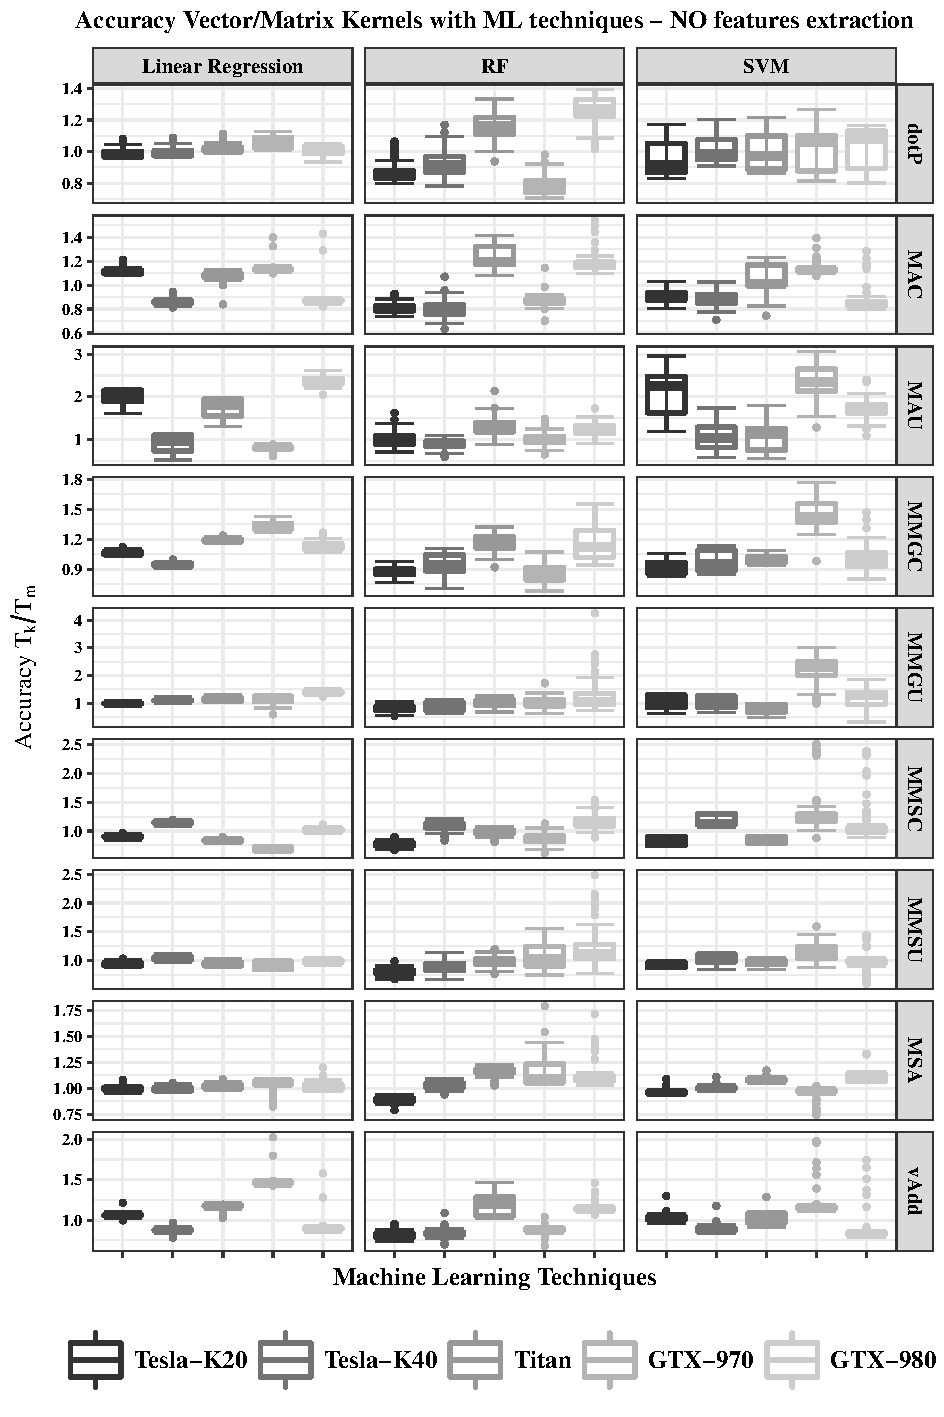
\includegraphics[scale=1]{images/ResultTechniques-fair.pdf}
    \caption{Accuracy}
    \label{fig:Results-NCA-Fair}
\end{figure}

\begin{figure}[htpb]
    \centering
    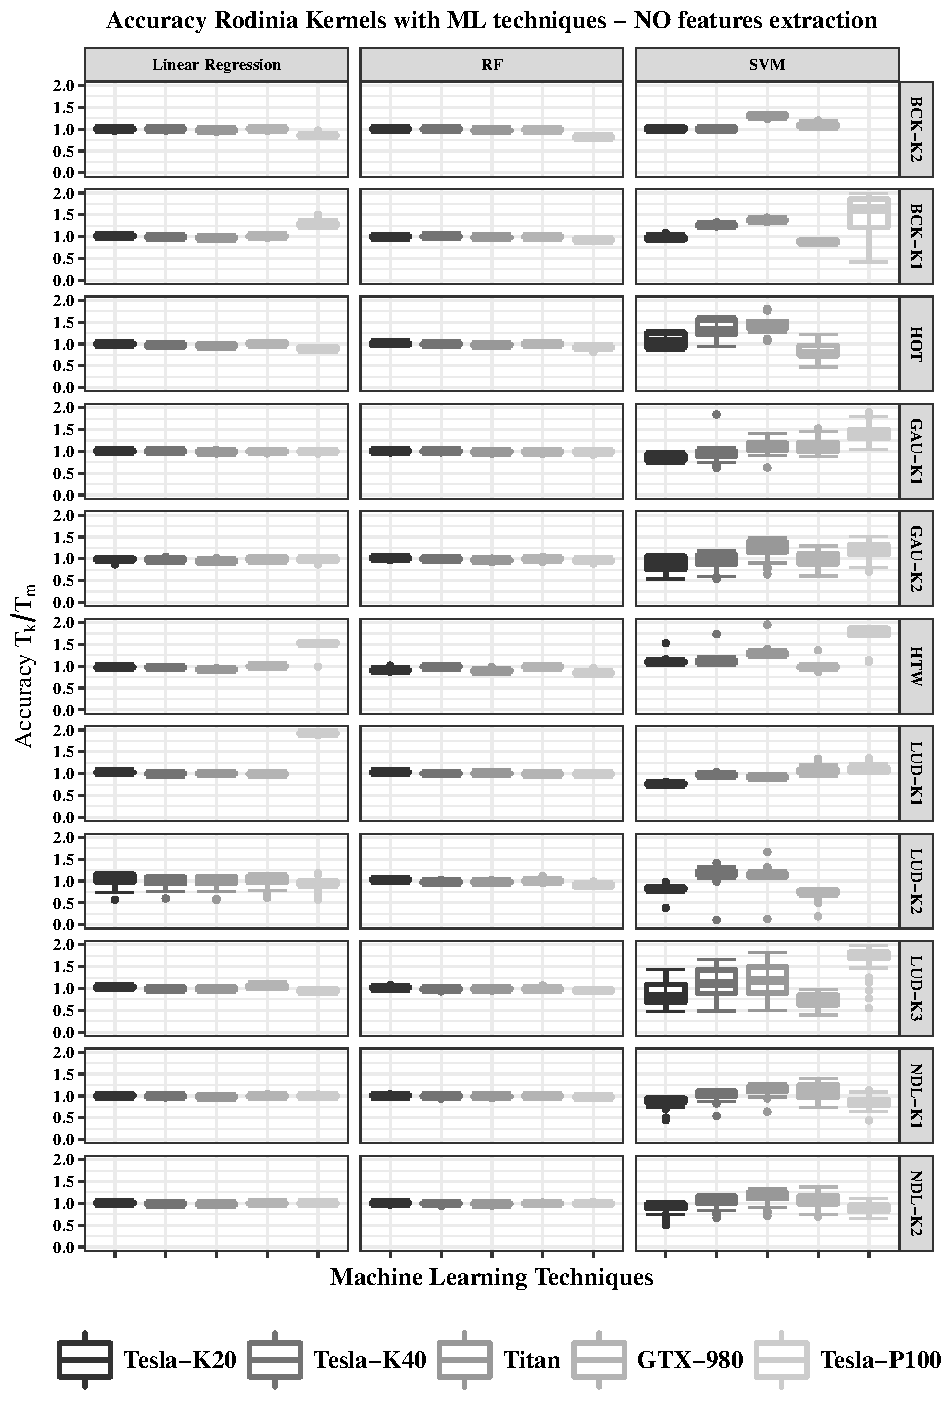
\includegraphics[scale=1]{images/ResultTechniques-Rodinia-fair.pdf}
    \caption{Accuracy}
    \label{fig:Results-RodiniaFair}
\end{figure}

Table~\ref{tab:MAPE:NCA} and \ref{tab:MAPE:Rodinia} shows the comparison between both analytical model and machine learning approaches in terms of Mean Absolute Percentage Error (MAPE). This table shows that both analytical model and machine learning techniques obtained reasonable predictions for almost all cases. 

% \todoRaph{Why you do not show the MAPE results for the AM? Even if they are large, I do not see any problem in showing them.} 

The Analytical model presented MAPE around of 5\% for almost all the vector/matrix applications. This adjustment with this $\lambda$ parameters will give us reasonable prediction until certain circumstances, in others the analytical model always will need calibration. Machine learning techniques can do better predictions whether more samples from each class of CUDA kernels and better features are determined.

\begin{table}[htpb]
\centering
\scalebox{1}{
\small
\begin{tabular}{| c | c | c  |  c | c |} 
\midrule%inserts double horizontal lines
\multirow{2}{*}{\textbf{Apps}}&\multicolumn{4}{c|}{\textbf{MAPE ML Techniques}}\\\cline{2-5}
&\textbf{AM}&\textbf{LR}&\textbf{SVM}&\textbf{RF}\\\midrule
MMGU & 3.75$\pm$5.14&16.47$\pm$13.40&23.06$\pm$16.85&10.44$\pm$9.82\\ \midrule
MMGC & 6.70$\pm$2.07&15.53$\pm$11.28&15.23$\pm$5.76&10.02$\pm$7.21\\ \midrule
MMSU & 5.15$\pm$2.19&5.33$\pm$1.93&15.36$\pm$9.64&4.84$\pm$1.94\\ \midrule
MMSC & 3.46$\pm$2.11&14.83$\pm$10.22&20.28$\pm$14.23&8.53$\pm$3.02\\ \midrule
MAU & 8.00$\pm$3.20&69.51$\pm$51.77&19.90$\pm$14.73&37.92$\pm$23.57\\ \midrule
MAC & 6.50$\pm$4.08&12.65$\pm$2.77&18.94$\pm$7.71&10.74$\pm$3.80\\ \midrule
dotP & 4.54$\pm$2.94&3.30$\pm$1.42&15.90$\pm$8.41&4.57$\pm$1.25\\ \midrule
vAdd & 3.58$\pm$2.00&18.98$\pm$16.56&15.11$\pm$6.76&8.72$\pm$4.51\\ \midrule
MSA & 3.00$\pm$1.22&2.99$\pm$1.73&10.64$\pm$4.95&5.81$\pm$4.23\\ \midrule\end{tabular}
}
\caption{MAPE of the different techniques used}
\label{tab:MAPE:NCA} 
\end{table}

\begin{table}[htpb]
\centering
\scalebox{.85}{
\begin{tabular}{|r|c|c|c|c|}
\hline\hline
\textbf{Kernels/Techn.} &\textbf{AM}& \textbf{LR}&\textbf{SVM}&\textbf{RF}\\ \hline
                         
BCK-K1 & 3.53$\pm$1.25&108.61$\pm$215.21&17.66$\pm$21.44&31.58$\pm$27.87\\ \midrule
BCK-K2 & 4.86$\pm$3.33&26.00$\pm$30.54&25.98$\pm$34.53&128.20$\pm$261.96\\ \midrule
GAU-K1 & 31.53$\pm$3.85&27.36$\pm$26.88&14.19$\pm$3.16&18.98$\pm$14.67\\ \midrule
GAU-K2 & 78.31$\pm$4.58&20.94$\pm$6.09&14.55$\pm$7.63&18.42$\pm$7.71\\ \midrule
HTW & 13.09$\pm$1.72&25.49$\pm$31.46&25.38$\pm$21.88&26.62$\pm$30.17\\ \midrule
HOT & 3.86$\pm$2.18&44.55$\pm$30.51&28.60$\pm$20.98&118.72$\pm$202.31\\ \midrule
LUD-K1 & - &3902028.92$\pm$8725176.99&11.20$\pm$11.63&11.03$\pm$7.73\\ \midrule
LUD-K2 & - &35.61$\pm$19.77&25.97$\pm$17.41&54.64$\pm$78.61\\ \midrule
LUD-K3 & - &46.53$\pm$34.59&18.57$\pm$10.46&43.78$\pm$33.70\\ \midrule
NDL-K1 & - &17.65$\pm$7.77&13.08$\pm$7.25&13.90$\pm$3.79\\ \midrule
NDL-K2 & - &15.18$\pm$2.86&10.82$\pm$3.85&13.40$\pm$3.49\\ \midrule
\end{tabular}}
\caption{MAPE of the prediction of the second context (in \%).}
\label{tab:MAPE:Rodinia}
\end{table}

\subsection{Results with extraction features}
We first performed the process of feature extraction. After applying the correlation and hierarchical clustering, we selected the 10 features below. The first 5 features are used in the experiments with 5 features, and the complete set is used for the experiments with 10 features.

\begin{lstlisting}[basicstyle=\small,numbers=none]
 elapsed_cycles_sm"                 
 [2] "gld_request"                       
 [3] "gst_request"   
 [4] "executed_control.flow_instructions"
 [5] "device_memory_read_transactions"                         
 [6] "active_cycles"                     
 [7] "global_store_transactions"         
 [8] "gst_inst_32bit"                    
 [9] "executed_load.store_instructions"  
[10] "misc_instructions"  
\end{lstlisting}

As it was mentioned in the last section we used two metrics, accuracy and Mean Absolute Percentage Error (MAPE) of the predictions of each machine learning algorithm. The accuracy is the ratio $t_k/t_m$, between the predicted times $t_k$ and the measured times $t_m$. MAPE is computed using equation~\ref{ec:MAPE}.

We evaluate the MAPE for each learning algorithm, linear regression (LR), support vector machine (SVM) and random forest (RF), when using 2 GPU parameters (number of cores and amount of L2 cache), when considering either 5 or 10 application features. We justify the selection of these 2 GPU parameters later in this section.

Table~\ref{tab:MAPE:Contex1} shows the MAPE for the ML algorithms for the first scenario, where we predict the execution time over a previously unseen GPU. %Blue and red cells represent the best and worst MAPE for each predicted GPU, respectively. Linear Regression obtained the best MAPE in 5 different GPUs, while Random Forests was better for the other 3 GPUs. Both LR and SVM benefited from using 10 features, while for RF it was better to use only 5 features. But overall, using LR with 5 features provided reasonably good predictions using a simple ML procedure and very few features. 



\begin{table}[htpb]
\centering
\scalebox{1}{
\small
\begin{tabular}{| c | c | c  |  c | c | c  |  c | } 
\midrule%inserts double horizontal lines
\multirow{2}{*}{\textbf{GPUs}}&\multicolumn{6}{c|}{\textbf{MAPE ML Techniques per Number of Features}}\\\cline{2-7}
&\multicolumn{2}{c|}{\textbf{LR}}&\multicolumn{2}{c|}{\textbf{RF}}&\multicolumn{2}{c|}{\textbf{SVM}}\\\midrule
& \textbf{5}&\textbf{10}& \textbf{5}&\textbf{10}& \textbf{5}&\textbf{10}\\\midrule
GTX-680 & 1.75&1.63&2.70&2.68&1.95&1.59\\ \midrule
Tesla-K40 & 1.24&1.10&0.73&0.69&1.63&1.46\\ \midrule
Tesla-K20 & 1.40&1.13&1.48&1.41&1.74&1.51\\ \midrule
Titan & 1.29&1.21&1.22&0.97&1.61&1.53\\ \midrule
Quadro & 2.62&2.24&3.23&3.16&2.89&2.34\\ \midrule
TitanX & 2.52&2.79&2.36&2.07&2.79&2.93\\ \midrule
GTX-970 & 2.00&2.41&2.93&2.88&2.26&3.10\\ \midrule
GTX-980 & 1.74&1.54&1.97&1.68&1.97&1.77\\ \midrule
Tesla-P100 & 3.71&4.49&7.89&8.36&4.06&4.23\\ \midrule
\end{tabular}
}
\caption{MAPE of the prediction of the first context (in \%). }
\label{tab:MAPE:Contex1} 
\end{table}

Table~\ref{tab:MAPE:Contex2} shows the MAPE of the ML algorithms when predicting the execution time of a previously unseen application. LM and SVM with 5 features obtained the best average MAPEs and seem appropriate choices for predicting the execution times. Although RF obtained the best MAPE for 6 kernels, it obtained poor MAPEs for some kernels, resulting in larger average MAPEs. Considering the results from both contexts (Tables~\ref{tab:context1} and Table~\ref{tab:context2}), it seems that using LR with 5 parameters is a better overall choice.


\begin{table}[htpb]
\centering
\scalebox{1}{
\small
\begin{tabular}{| c | c | c  |  c | c | c  |  c |} 
\midrule%inserts double horizontal lines
\multirow{2}{*}{\textbf{Kernels}}&\multicolumn{6}{c|}{\textbf{MAPE ML Techniques per Number of Features}}\\\cline{2-7}
&\multicolumn{2}{c|}{\textbf{LR}}&\multicolumn{2}{c|}{\textbf{RF}}&\multicolumn{2}{c|}{\textbf{SVM}}\\\midrule
& \textbf{5}&\textbf{10}& \textbf{5}&\textbf{10}& \textbf{5}&\textbf{10}\\\midrule
BCK-K1&2.07&2.11&1.64&1.88&2.69&1.78\\ \midrule
BCK-K2&2.87&2.62&3.25&2.97&2.46&2.69\\ \midrule
GAU-K1&3.98&4.60&3.36&3.59&9.49&9.29\\ \midrule
GAU-K2&1.50&1.80&9.36&6.61&8.02&11.30\\ \midrule
HTW&3.78&2.86&6.51&5.43&4.52&4.74\\ \midrule
HOT&2.56&2.40&2.57&2.35&10.12&8.01\\ \midrule
LUD-K1&4.02&4.18&2.13&4.19&15.72&15.36\\ \midrule
LUD-K2&1.88&2.09&2.16&3.19&2.28&2.42\\ \midrule
LUD-K3&0.98&1.17&1.83&1.93&1.48&1.44\\ \midrule
NDL-K1&1.14&1.18&0.54&0.49&1.65&1.93\\ \midrule
NDL-K2&1.03&1.01&0.47&0.50&1.59&1.91\\ \midrule
MAU&2.18&3.87&13.22&10.73&13.37&14.38\\ \midrule
MAC&1.38&1.37&1.91&2.10&2.07&1.72\\ \midrule
dotP&2.47&10.88&8.42&6.11&9.38&12.44\\ \midrule
vAdd&2.93&4.25&3.95&2.57&2.54&2.96\\ \midrule
MSA&18.65&12.14&41.22&39.03&48.19&39.53\\ \midrule


\end{tabular}
}
\caption{MAPE of the prediction of the second context (in \%). }
\label{tab:MAPE:Contex2} 
\end{table}

For each context, we also tested the number of GPU parameters (features) to use. Figure~\ref{fig:GPUParam} shows the average MAPE of the linear regression model with different numbers of GPU parameters in both contexts. Figure~\ref{fig:GPUParam-RF} show the average MAPE of the random forest with different numbers of GPU parameters in both contexts. We can see that 2 parameters provided the smaller error for 5 application features. For 10 features, including more parameters decreased only slightly the average MAPE for linear regression model, increased for random forests. Consequently, we decided to use 2 GPU parameters in the experiments. The evaluated GPU parameters are shown below, ordered from higher to lower Spearman coefficient against execution times.

\begin{lstlisting}[basicstyle=\small, numbers=left, stepnumber=1]
L2
num_cores_sm
memory_clock
compute_version
theoretical_flops
max_clock_rate
\end{lstlisting}

\begin{figure}[htpb]
    \centering
    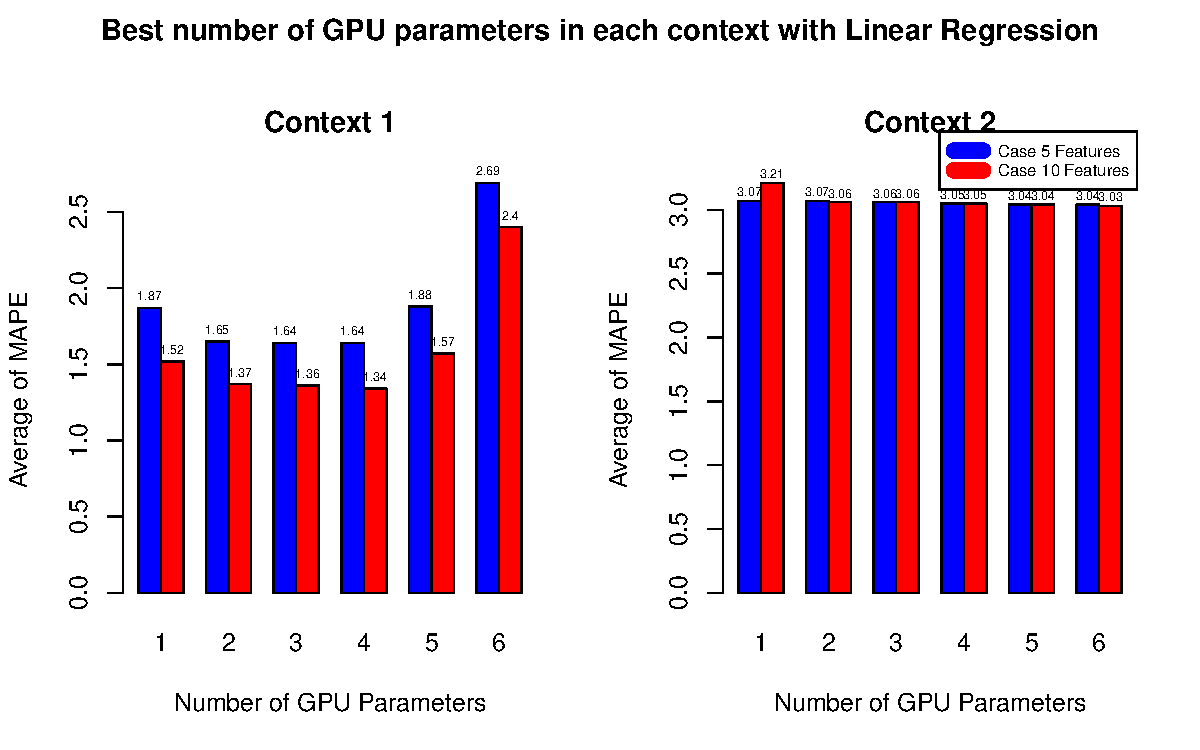
\includegraphics[scale=.75]{./images/parameters.pdf}
    \caption{Best number of GPU parameters in each one of the contexts for Linear Regression}
    \label{fig:GPUParam}
\end{figure}

 
\begin{figure}[htpb]
    \centering
    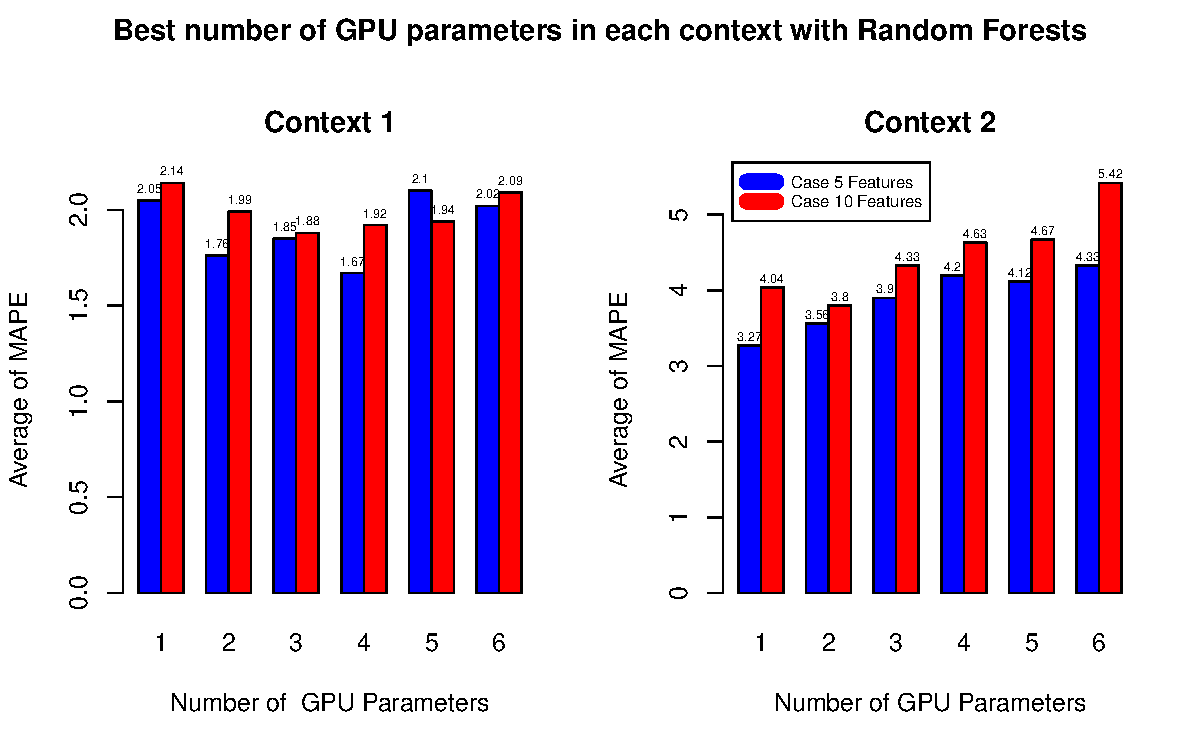
\includegraphics[scale=.75]{./images/parameters-RF.pdf}
    \caption{Best number of GPU parameters in each one of the contexts for Random Forests}
    \label{fig:GPUParam-RF}
\end{figure}


Figures~\ref{fig:Results-contex1},  \ref{fig:Results:context2:NCA} and \ref{fig:Results:context2:Rodinia} show box plots of the accuracies of individual samples for the first scenario of GPUs and second scenario of vector matrix CUDA kernels and second scenario of Rodinia CUDA kernels, respectively. The boxes represent the median and the upper and lower first quartiles, with whiskers representing the maximum and minimum possible errors. Outliers are marked as individual points.

\begin{figure}[htpb]
    \centering
    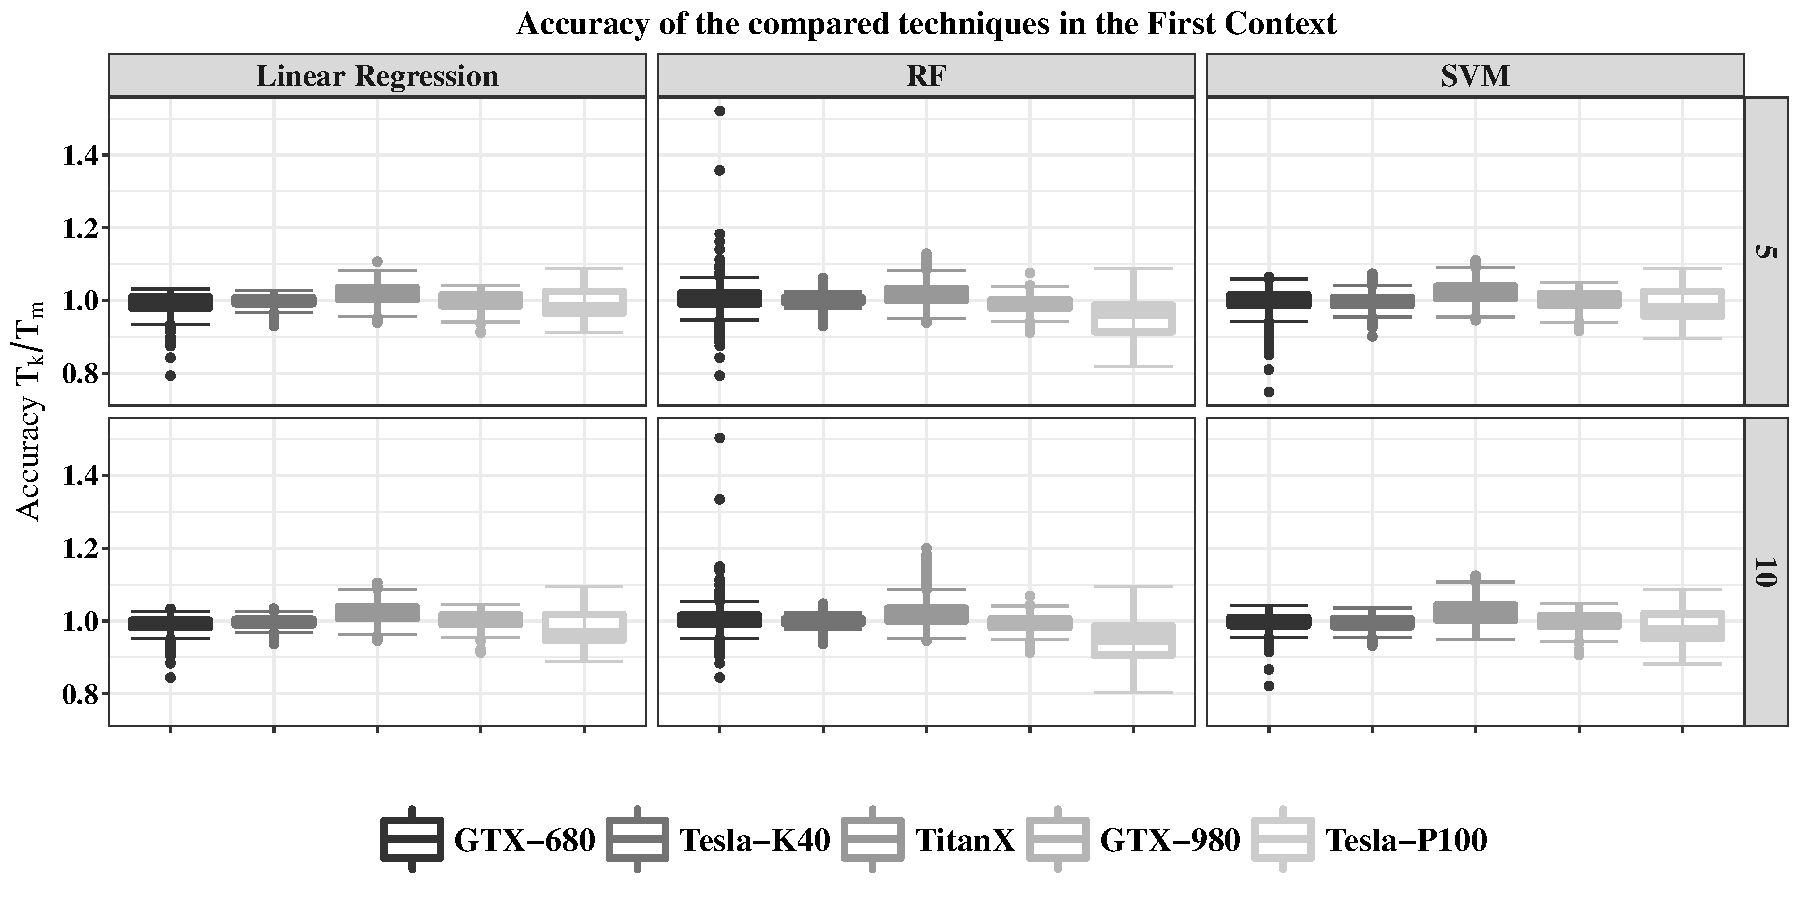
\includegraphics[scale=.5]{images/ResultTechniques-Context1.pdf}
    \caption{Accuracy ($t_k/t_m$) of the first scenario with GPUs of 3 different architectures}
    \label{fig:Results-contex1}
\end{figure}

\begin{figure}[htpb]
    \centering
    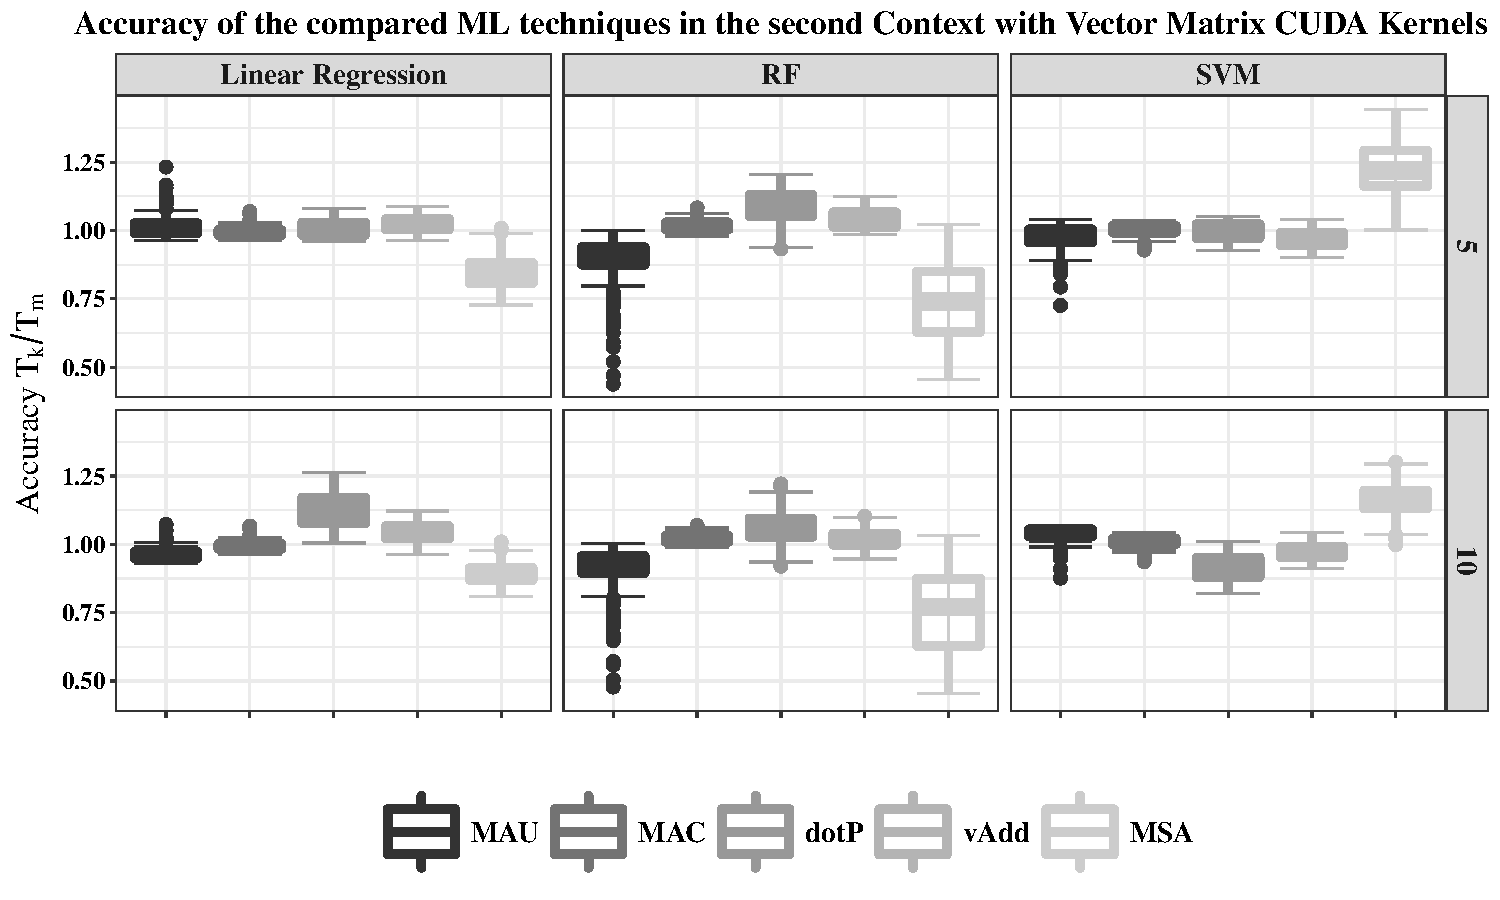
\includegraphics[scale=.65]{images/ResultTechniques-Context2-NCA.pdf}
    \caption{Accuracy of the 5 vector/matrix CUDA kernels used in the second scenarios}
    \label{fig:Results:context2:NCA}
\end{figure}

\begin{figure}[htpb]
    \centering
    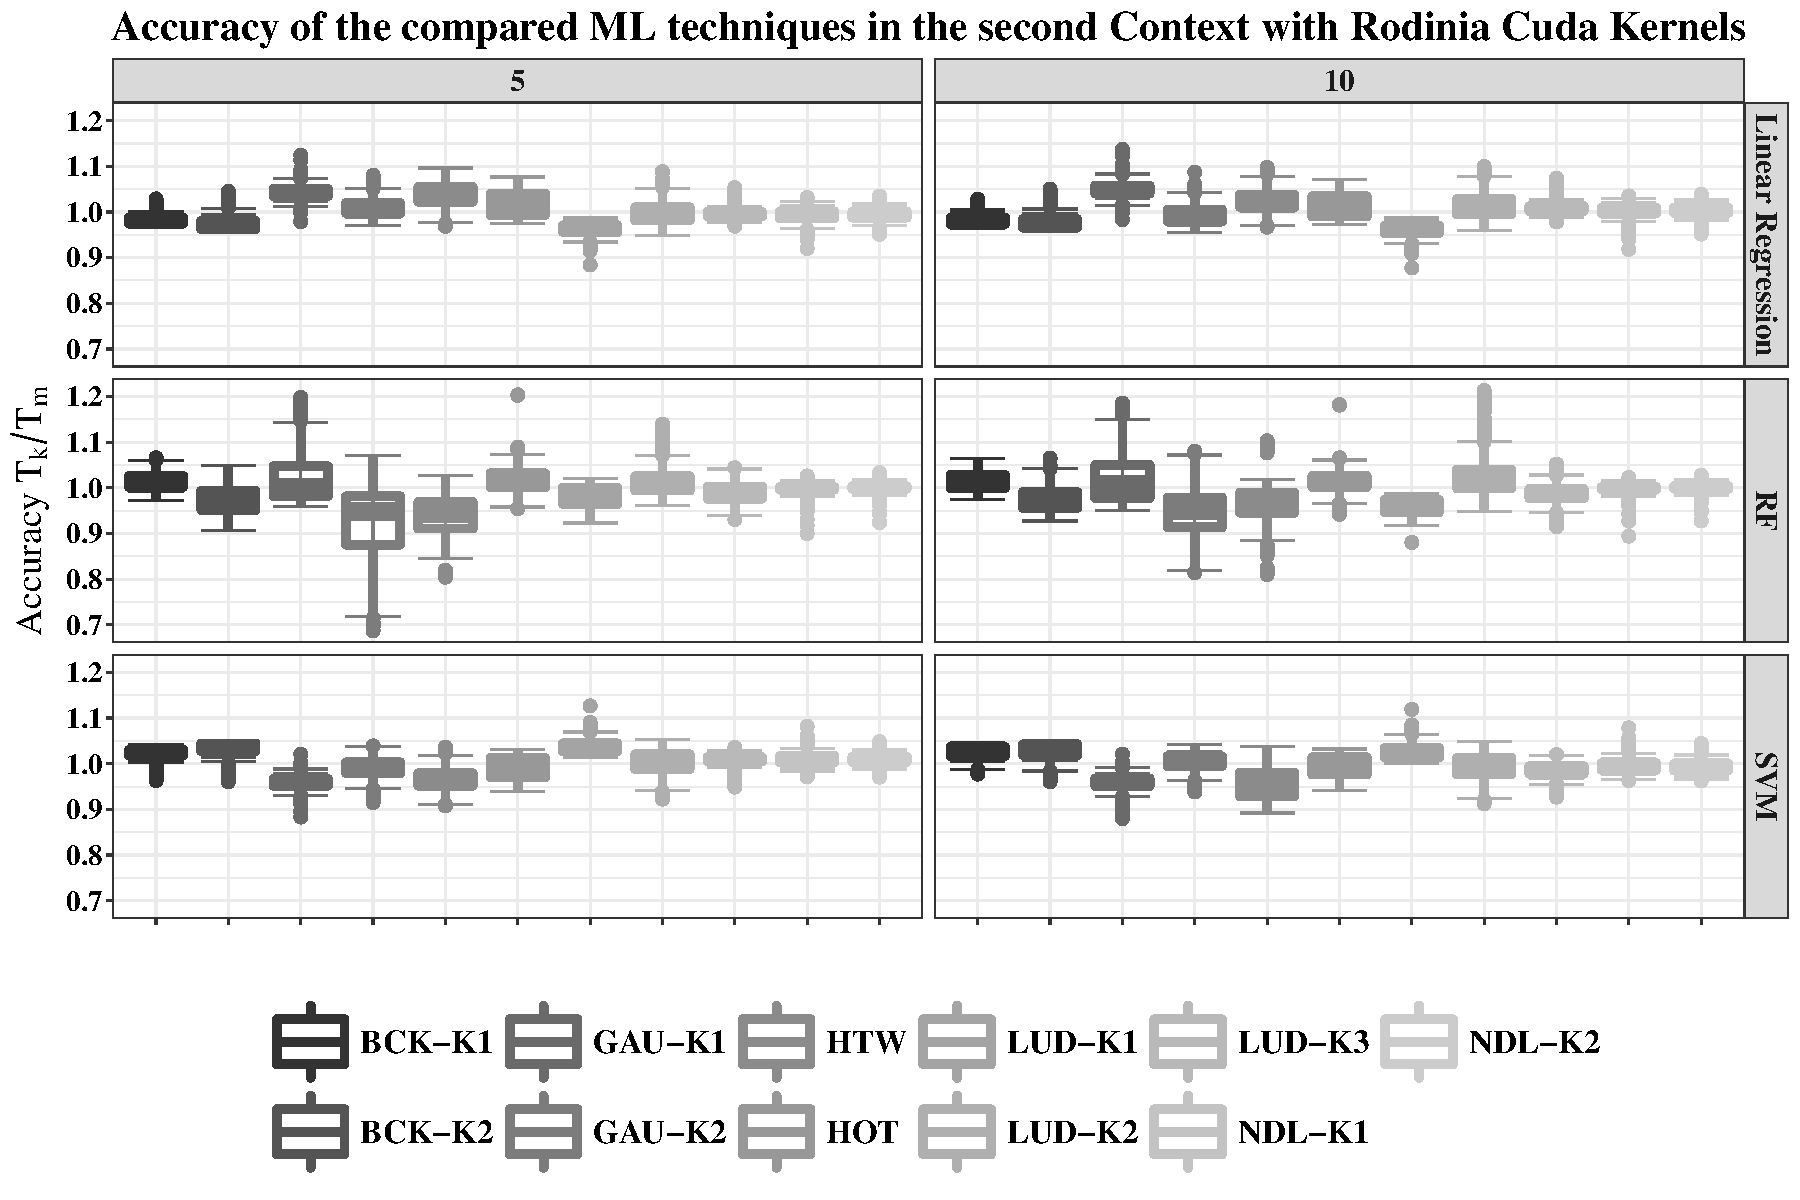
\includegraphics[scale=.5]{images/ResultTechniques-Context2-Rodinia.pdf}
    \caption{Accuracy of the second scenarios of the Rodinia CUDA kernels}
    \label{fig:Results:context2:Rodinia}
\end{figure}

Overall, the predictions for the first context (Figure~\ref{fig:Results-contex1}) was good, with the most samples with a accuracy between 0.9 and 1.1. For the second context (Figure~\ref{fig:Results:context2:NCA} and ~\ref{fig:Results:context2:Rodinia}) the predictions were less accurate for some kernels, but for the SVM and linear regression they were still mostly between 0.85 and 1.15. SVM and LR obtained similar accuracies because we used a linear kernel for SVMs, since it provided than using nonlinear kernels, such as polynomial, Gaussian (RBF) and sigmoid. For Random Forests, we set the number of trees to $50$, and the number of predictor candidates at each split to $3$, as these values resulted in better predictions and faster executions. 
